\section{Literaturrecherche}
Die folgenden Schritte wurden unternommen: TODO

\renewcommand{\arraystretch}{1.5}
\begin{table}[htp]
\centering
\begin{tabular}{l|p{3.5cm}|l|p{3.5cm}}
Resourcentyp & Resource & Datum & Suchergebnisse\\
\hline
Literaturdatenbank & DHBW & 26.02.2013 & TODO benutzbare Ergebnisse\\
Literaturdatenbank & Deutsches Patent- und Markenamt & 26.02.2013 & TODO\\
Internetquelle & Google & 27.02.2013 & TODO\\
Internetquelle & Wikipedia & 02.03.2013 & TODO\\
\end{tabular}
\end{table}
\section{Bibliothek der DHBW Stuttgart}
Die Hochschulbibliothek der DHBW Stuttgart\footnote{http://www.dhbw-stuttgart.de/themen/service-einrichtungen/bibliothek.html} bietet einen Bibliothekskatalog der online\footnote{https://bsz.ibs-bw.de/aDISWeb/app?service=direct/0/Home/\$DirectLink&sp=S127.0.0.1:23412} durchsucht werden kann. Es wird eine Volltextsuche verwendet. Eine Suche nach \glqq Java\grqq ~ergab 22 Treffer. Eine Suche nach \glqq Java 7\grqq ~ergab 5 Treffer.

\begin{center}
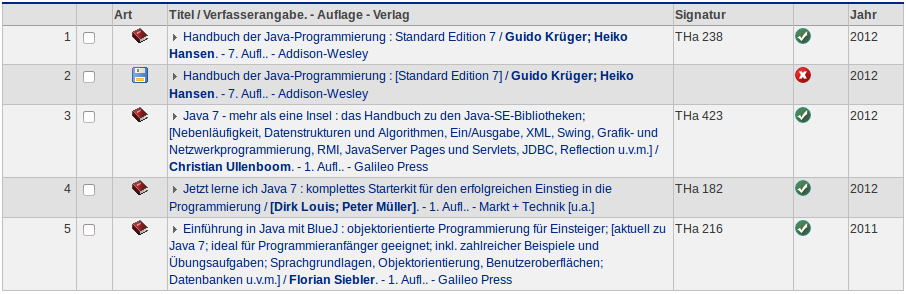
\includegraphics[width=\textwidth]{images/dhbw-lib-search-results.png}
\end{center}

Wir haben alle gelisteten Bücher zu Java 7 vor Ort in der Bibliothek gesichtet. Von den gelisteten Exemplaren ging nur ein Werk\cite{javainsel2} direkt auf die Neuerungen in Java 7 ein. Die anderen Fachbücher stellen eine allgemeine Beschreibungen der Java SE Bibliotheken dar denen lediglich Java in Version 7 zu Grunde liegt\cite{dhLibHandbuchJava} oder Sie richten sich gezielt nur an Javaanfänger\cite{dhLibJetztJavaLernen}\cite{dhLibBlueJStart}, wodurch sie für eine weitere Betrachtung im aktuellen Kontext nicht interessant sind.\\

Das Buch \glqq Java 7 - Mehr als eine Insel\grqq\cite{javainsel2} ~beschreibt in einem eigenen Kapitel die Neuerungen in Java 7. Der Autor, Christian Ullenboom, ist uns bereits durch seine frühere Veröffentlichung \glqq Java ist auch eine Insel\grqq\cite{javainsel1} ~bekannt gewesen, die mittlerweile als Referenzwerk für die Java SE Bibliotheken gehandelt wird. Die aktuelle Ausgabe dieses Buchs basiert ebenfalls auf Java 7 und kann im \glqq Stand der Technik\grqq ~Dokument verwendet werden.
\renewcommand{\arraystretch}{1}
%
%eof

